\documentclass{book}
\usepackage[german]{babel}
\usepackage[utf8]{inputenc}
\usepackage[T1]{fontenc}
\usepackage{pdfpages}


\title{Design Document}
\author{\"Ozlem  Ay \and Georg Engler \and Gohar
Samvelyan \and Nils Sommer}
\date{\today}


\begin{document}
\frontmatter
\maketitle
\tableofcontents
\mainmatter
\part{Low Level Design}

\chapter{Einleitung}
 In diesem Dokument wird das Low Level Design unseres Systems näher erläutert.
 Als Basis unseres Entwurfes dient das Muster Architektur Design. Mithilfe von Graphiken
 und Erläuterungen wird die Systemstruktur unseres Systems verdeutlicht. Ausgehend von der 
 groben Struktur des Architektur Designs wurde mit Hilfe von verschiedenen Pattern ein Programmstuktur
 entwickelt, sodass im nächsten Schritt nur noch die Implementierung der zur Verfügung gestellten
 Methoden erfolgen muss.
 
\chapter{Programmstruktur}

\section{Programmaufbau}
Grob lässt sich unser Programm in die Verwaltung und die rechnende Komponente unterteilen.
In der Verwaltung werden Nutzer, Pakete, Modelle, Daten verwaltet und geordnet. In der rechnenden
Komponente erfolgt die Ausführung der Algorithmen. 

\section{Verwaltung}
Die Nutzerverwaltung dient zur Loginverwaltung und der Prüfung von Zugriffsrechten. Durch Zugriff auf die 
Nutzerdatenbank kann über die Nutzerverwaltung erfahren werden ob es sich bei einem Nutzer um einen Admin oder
nur einen regrestierten Nutzer handelt. Da bestimmte Operationen, wie das löschen von Nutzern oder ändern von
Nutzer Daten, nur von einem Admin oder dem Nutzer  durchgeführt werden können, müssen zuerst Zugriffsrechte geklärt werden. Hier wird das Proxy Pattern verwendet, sodass vor bestimmten Anfragen die Rechte bei der eigentlichen Nutzerverwaltung abgefragt werden.\\
Jede Nutzer ID ist einzigartig und dient dazu alle Daten der Nutzer über diese Abrufen zu können. Die Nutzer ID entspricht dem Namen des Nutzers den er zum Login verwendet. Um die Einzigartigkeit jeder Nutzer ID zu gewährleisten wird bei jedem neuen Nutzer der sich regrestiert geprüft ob seine ID bereits vorhanden ist. \\
Die Nutzerverwaltung hat Zugriff auf die Nutzerdatenbank, in der sämtliche Informationen über jeden Nutzer (z.B Passwort oder Pakete) gespeichert sind.
\\
Die Paketverwaltung verwaltet den Zugriff auf Pakete. Auch hier kommt das Proxy Pattern zum Einsatz um bei allen Anfragen zuerst zu klären, ob der entsprechende Nutzer zugriff auf das jeweilige Paket hat. Über den Paketverwaltungs Proxy wird zusätzlich der Zugriff auf die Pakete gesichert. Für jede Anfrage wird die Nutzer ID benötigt unter welcher in der Nutzer Datenbank die Pakete des Nutzers gelistet sind.
Der Haupnutzer eines Paketes ist der Besitzer und Ersteller des Paketes. Im Rahmen eines Paketes übernimmt er die Rolle des Admin.\\
\\
Modelle können nur in Paketen gespeichert werden. Somit beinhaltet jedes Paket Null oder mehrere Modelle, welche über die Paketverwaltung auf lokale Computer heruntergeladen werden können.
Modelle speichern durch welchen Algorithmus und welchen Datensatz sie erstellt wurden. So kann ein Nutzer gewarnt werden falls er nochmal das gleiche Modell versucht zu erstellen.

\section{rechnende Komponente}
Für das Ausführen der Algorithmen und das Erstellen der Modelle wurde das Micro Kernel Design aus dem Architektur Design übernommen. Das Proxy Design Pattern wurde auch hier für den Adapter verwendet um vor jeder Anfrage die Zugriffsrechte zu klären. Der Adapter selber speichert die aktuelle Anzahl an Berechnungen um diese im Notfall zu begrenzen. \\
\\
Um einen Algorithmus Auszuführen initialisiert der Adapter einen Mikro Kern. Der Externe Server übergibt dem Mikro Kern die Algorithmus ID und die Daten ID. Über den Internen Server lädt der Mikro Kern die Daten und den Algorithmus. Der Interne Server hat Zugriff auf die RDF Datenbank aus der er die Daten liest und dem Mikro Kern übergibt. Das erzeugen der Algorithmen wird mithilfe des Factory Patterns verwirklicht. So kann der Interne Server die Algorithmen Instazieren und an den Mikro Kern zurück geben. Dieser gibt Daten und Algorithmen an den Externen Server wo die Berechnung stattfindet.\\
\\
Da die Möglichkeit besteht eigene Algorithmen zuzufügen müssen alle Algorithmen ein Interface implementieren.
Dieses fordert von den Algorithmen die Bereitstellung der Methode start, über die die Berechnung gestartet werden kann. Von Anfang an werden die Algorithmen j48, Random Forrest und smo zur Verfügung gestellt. \\
\\
Alle Anfragen des Client werden von der REST Schnittstelle bearbeitet und weitergeben. Die REST Schnittstelle wird mit einem vorgefertigten Servlet verwirklicht (z.B. Jersey).\\
Bei Fuseki handelt es sich um den SPARQL Endpoint und arq ist die Anfrage Engine. Beide stammen aus dem ofiziellen Apache jena Framework.

\section{Klassendiagramm} 
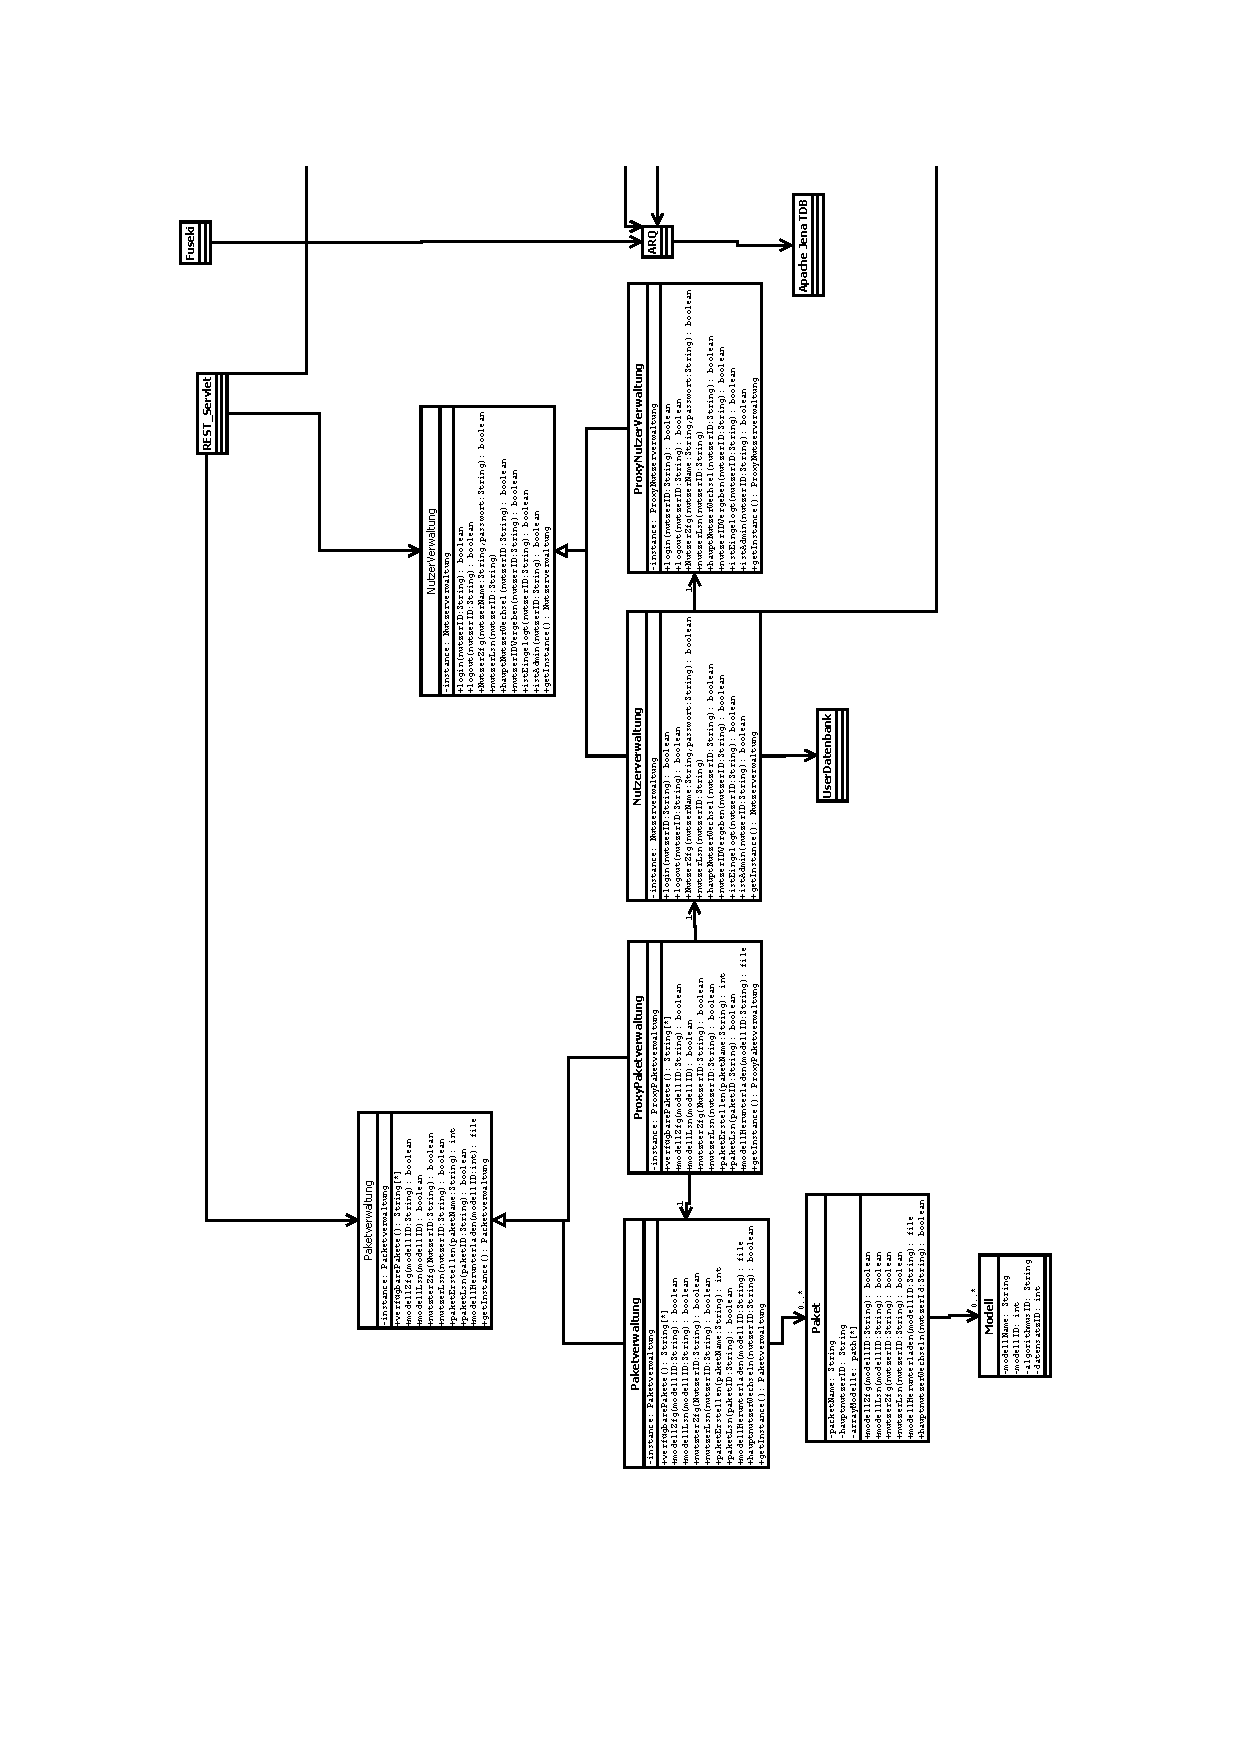
\includepdf[pages = 1-2]{Klassendiagramm.pdf}

\chapter{Nicht genutzte Pattern}
 
\section{Master Slave}
Master Slave haben wir nicht verwendet da nirgendwo in unserem Programm genügend große Aufgaben bewältigt werden damit sich ein Aufteilen der Aufgaben lohnen würde. 

\section{View Handler}
View Handler wurde nicht verwendet da unser Programm nur über die REST Schnitstelle kommuniziert und so nicht zwischen verschieden Views gewechselt werden muss.

\section{Forwarder Receiver}
Forwarder Reciver wurde nicht verwendet da nirgendwo im Programm eine Kommonikation zwischen zwei paaren statt findet. 

\section{Command Processor}
Der Command Processor wurde nicht verwendet, da es keinen Vorteil bringt einzelne Kommandos zu programmiern über die Methoden auf andere zugreifen können. Weiter wird in unserm Programm kein Schritt dierekt rückgängig gemacht,
sodass der Vorteil des Undo Kommandos nicht benötigt wird. 

\section{Observer Pattern}
Das Observer Pattern wurde nicht verwendet da kein Objekt auf eine Veränderung eines anders Objektes wartet.


\chapter{Erläuterung der Klassen und ihrer Methoden}

\section{Allgemein}
Im ganzen Dokument wurden keine Getter, Setter und Konstruktoren aus Übersicht Gründen erwähnt. Sie haben keine wichtige Funktion für das Design, weshalb sie unerwähnt bleiben können, dennoch müssen sie Implementiert werden.
\section{Nutzerverwaltung}
Die Nutzerverwaltung hat Zugriff auf die Nutzerdatenbank und dient zur Abfrage von Zugriffsrechten.\\
\\
login: Login von Usern \\
logout: logout von Usern\\
nutzerZfg: regrestieren neuer Nutzer\\
nutzerLsn: löschen von Nutezrn\\
hauptNutzerWechsel: Wechsel des Haupnutzers in einem Paket\\
nutzerIDVergeben: gibt zurück ob eine Nutzer ID schon vergeben ist\\
istEingelogt: gibt zurück ob ein Nutzer eingelogt ist, wenn ja ist er auch ein regrestierter Nutzer
istAdmin: gibt zurück ob der Nutzer Adminrechte hat

\section{Paketverwaltung}
Die Paketverwaltung kümmert sich um die Verwaltung von Paketen und die Zugriffe auf die Methoden des Paketes\\
\\
verfügbare Pakete: liefert alle für den Nutzer nutzbare Pakete zurück\\
modellZfg: neues Modell zu einem Paket hinzufügen\\
modellLsn: ein Modell aus einem Paket entfernen\\
nutzerZfg: einen neuen Nutzer zum Paket zufügen\\
nutezrLsn: einem Nutzer die Zugriffsrechte entziehen\\
paketErstellen: ein neues Paket erstellen\\
modellHerunterladen: ein Modell aus einem Paket herunterladen.\\

\section{Paket}
Ein Paket dient zum Speichern und austauschen von Modellen.\\
\\
Methoden siehe Paketverwaltung.

\section{Modell}
Ein Modell welches  durch einen Algorithmus erstellt wurde.

\section{Adapter}
Der Adapter ist die Schnittstelle zur Berechnung von Modellen.\\
\\
initialisiere: initialisiert einen neuen Mikrokern.\\
pluginAnfrage: übergibt Daten ID und Algorithmus ID um die Modellerstellung zu starten.

\section{Mikrokern}
Der Mikro Kern lädt über den internen Server die Daten und den Algorithmus.\\
\\
ladeAlgoroithmus: fordert Internen Server zum laden des Algorithmus auf.\\
ladeDaten: fordert Internen Server zum laden der Daten auf.

\section{Externer Server}
Auf dem Externen Server werden die Algorithmen ausgeführt.\\
\\
laden: zum laden von Algorithmus und den Daten.\\
erstelleModell: ausführen des Algorithmus.
 
\section{Interner Server}
Der Interne Server läd auf Anfrage den Algorithmus und dei Daten aus der Datenbank.\\
\\
ladeAlgorithmus: zuzm laden des Algorithmus.\\
ladeDaten: lädt Daten aus der Datenbank.

\section{IAlgorithmus}
Das Interface IAlgorithmus muss von alle Algorithmen implementiert werden.\\
\\
start: zu Starten der Berechnung.

\section{InstanziiereAlgo}
Die Klasse Instanzieiiere Algo dient nur zum instanziieren eine Algorithmus.\\
\\
instanziieren: zum instanziieren eines Algorithmus.

\chapter{Sequenzdiagramme}

\section{Einloggen eines Nutzers}
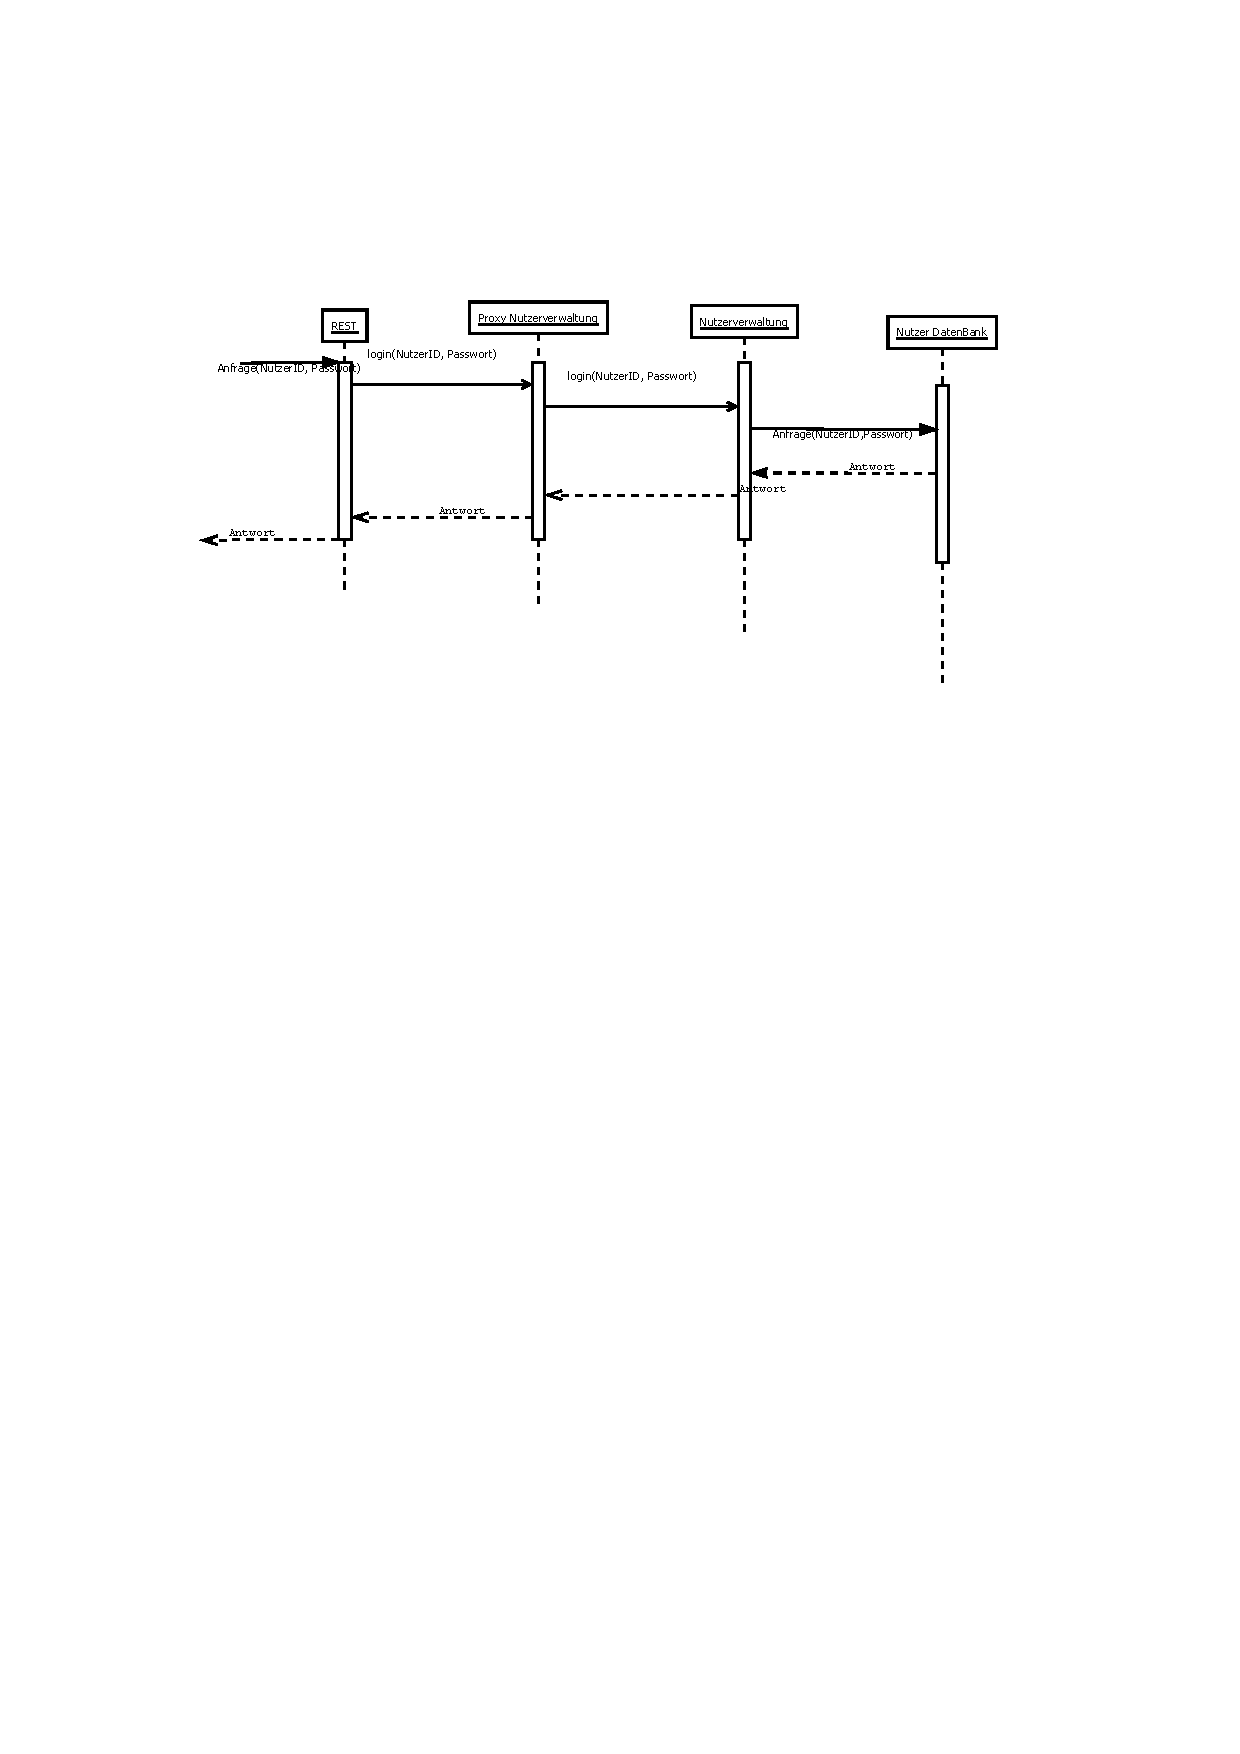
\includepdf{loginSequenz.pdf}

\section{Erstellen eines Modells}
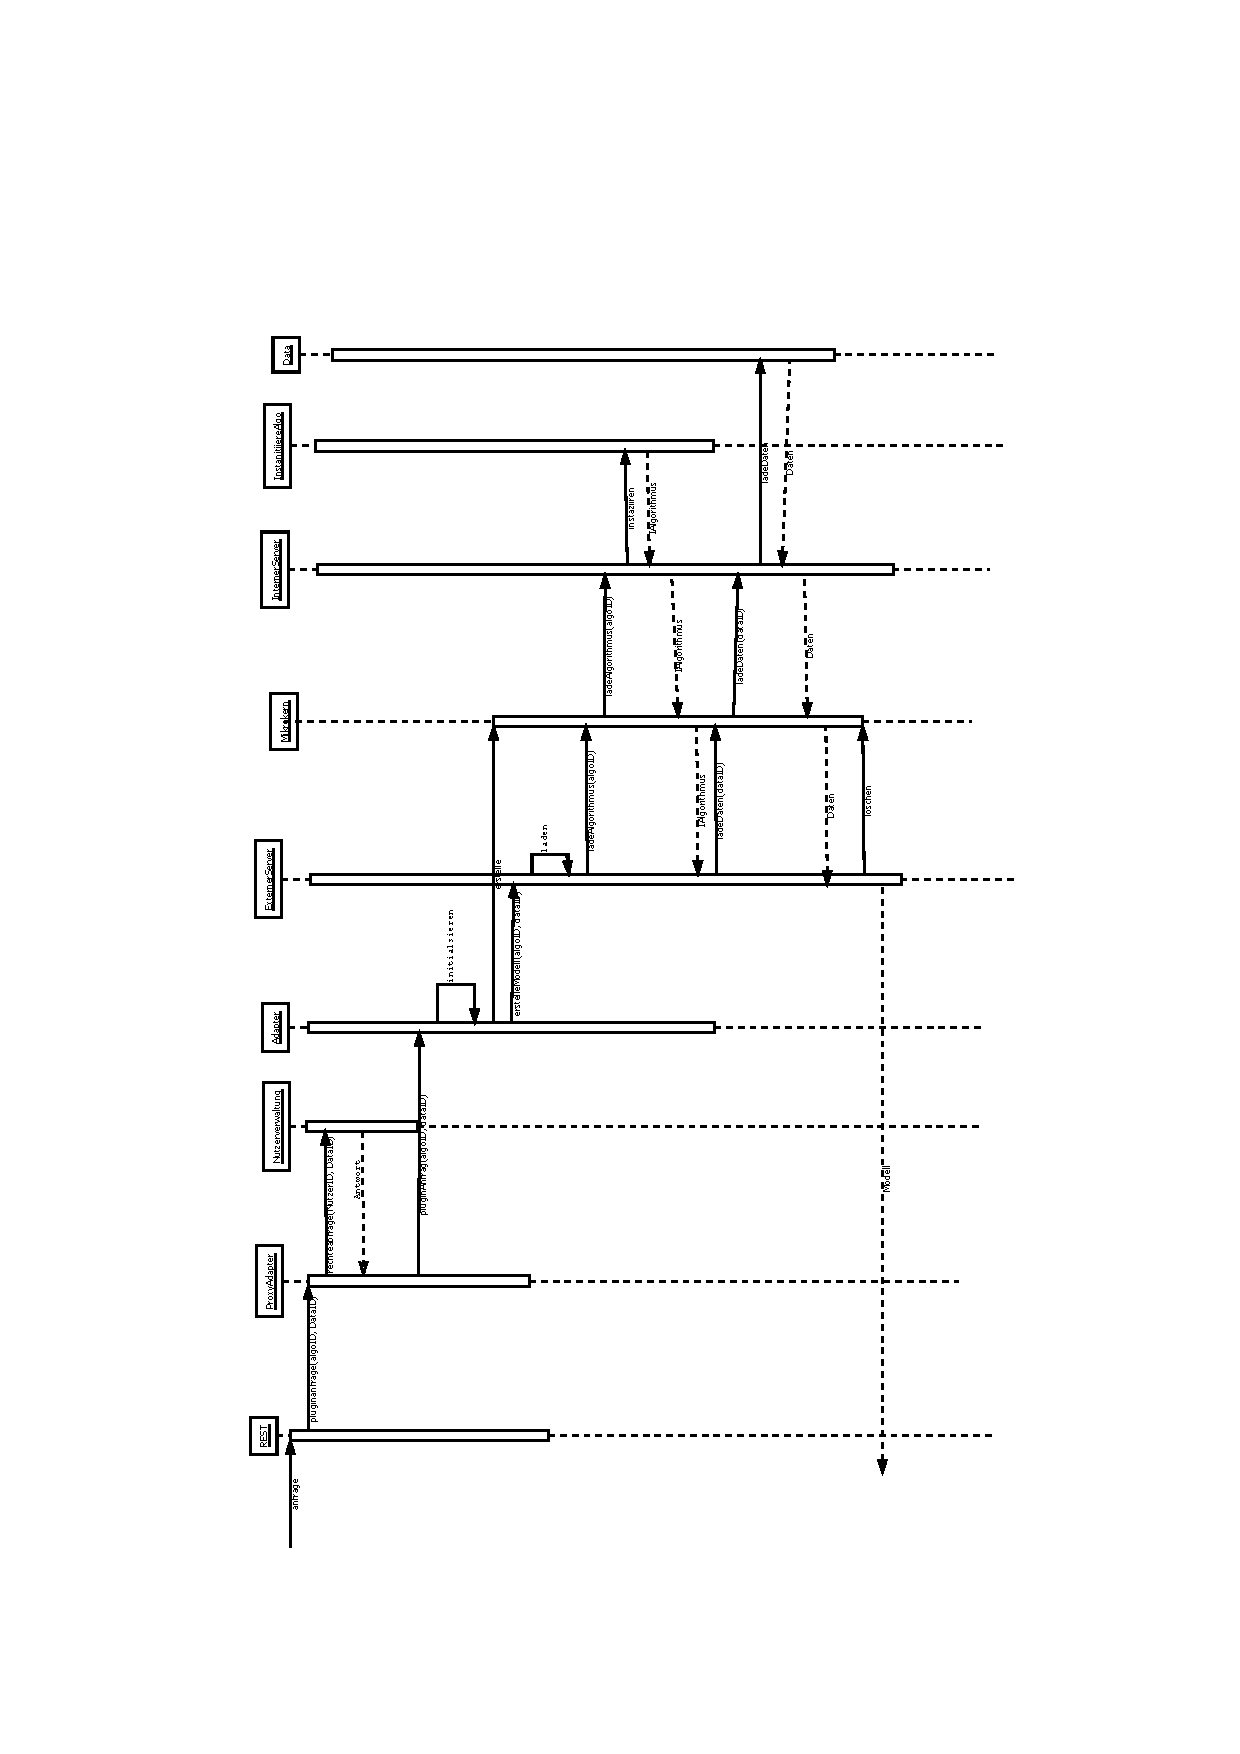
\includepdf{ModellErstellenSequenz.pdf}

\end{document}

%%% Local Variables:
%%% mode: latex
%%% TeX-master: t
%%% End:
